\documentclass[a4paper]{article}

\usepackage[utf8]{inputenc}
\usepackage[spanish]{babel}
\usepackage{graphics}
\usepackage{caption}
\usepackage{subcaption}
\usepackage[demo]{graphicx}
\usepackage{enumitem}
\usepackage{longtable}
\usepackage{listings}
\usepackage{listingsutf8}
\usepackage{framed}
\usepackage{float}
\usepackage{hyperref}

\begin{document}

\title{Informe del sistema de recuperación tradicional MiniTREC}
\author{
	Jaime Ruiz-Borau Vizárraga\\
	\texttt{546751}
	\and
	Alberto Sabater Bailón\\
	\texttt{546297}
	}
\date{}
\maketitle

\section{Arquitectura del software desarrollado}
\paragraph{}El siguiente diagrama de clases representa el diseño arquitectural del software desarrollado para el sistema de recuperación tradicional:
\begin{figure}[!hb]
	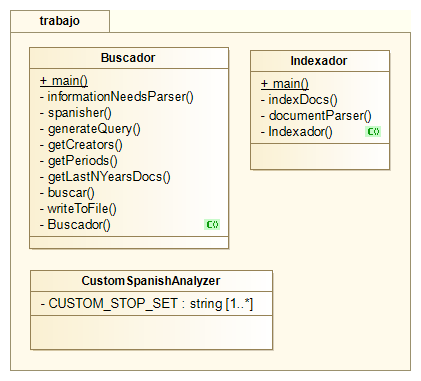
\includegraphics[width=\linewidth]{DiagramClass.png}
	\caption{Diagrama de clases y paquetes del sistema}
	\label{fig:class}
\end{figure}
\\
\newpage
\paragraph{}Como se puede apreciar en el diagrama, todas las clases se alojan en el paquete \textbf{trabajo}. Los nombres de las principales clases se explican por sí mismos: la clase \textit{Indexador} es la que posee métodos para indexar una colección de documentos especificada por parámetro tal y como solicita el enunciado; y la clase \textit{Buscador} es la que se encarga de realizar las consultas de las necesidades de información en base al índice creado por la clase Indexador.
\paragraph{}Adicionalmente existe una tercera clase, \textit{CustomSpanishAnalyzer}, que extiende a la clase de Lucene \textbf{Analyzer}. Reimplementa el método \textit{createComponents}, que permite modificar las StopWords que suprimirá el analizador a la hora de lematizar una consulta.

\section{Técnicas empleadas}
\subsection{Técnicas empleadas en el Indexador}
\paragraph{}Dada la naturaleza de la colección de documentos del Zaguán, se ha optado por realizar un análisis de las etiquetas de los documentos extrayendo la información de todas ellas siguiendo el estándar de la iniciativa Open Archives \textbf{(Open Archives Initiate)}. Dicho estándar establece una serie de etiquetas en documentos XML: \textbf{Title} \textit{(título)}, \textbf{Creator} \textit{(autor)}, \textbf{Subject} \textit{(materia)}, \textbf{Description} \textit{(descripción)}, \textbf{Publisher} \textit{(editor)}, \textbf{Contributor} \textit{(asistente)}, \textbf{Date} \textit{(fecha)},
\textbf{Type} \textit{(tipo)}, \textbf{Format} \textit{(formato)}, \textbf{Identifier} \textit{(identificador)}, \textbf{Source} \textit{(fuente)}, \textbf{Language} \textit{(idioma)}, \textbf{Relation} \textit{(relacion)}, \textbf{Coverage} \textit{(cobertura)} y \textbf{Rights} \textit{(derechos)}.
\paragraph{}Aunque varios de ellos no aparecen en la colección de documentos del Zaguán, se implementaron igualmente su análisis y extracción en el caso de que en el futuro se llegasen a incluir en los documentos del Zaguán (mayor modularidad futura).
\paragraph{}Para cada etiqueta descrita anteriormente, simplemente se crearon los campos asociados con el mismo nombre y lo siguientes tipos:
\begin{itemize}
	\item \textbf{TextField} - Title, Creator, Subject, Description, Publisher y Contributor
	\item \textbf{IntField} - Date
	\item \textbf{StringField} - Type, Format,
\end{itemize}


\section{Puntos tratados}

\section{Otros puntos}

\end{document}